\chapter{Hiện thực giao tiếp không dây cho node cảm biến}
\section{Giới thiệu}
Sử dụng công nghệ truyền thông không dây LoRa \cite{tl12} (Long Range Radio).\\
\begin{center}
\begin{figure}[htp]
\begin{center}
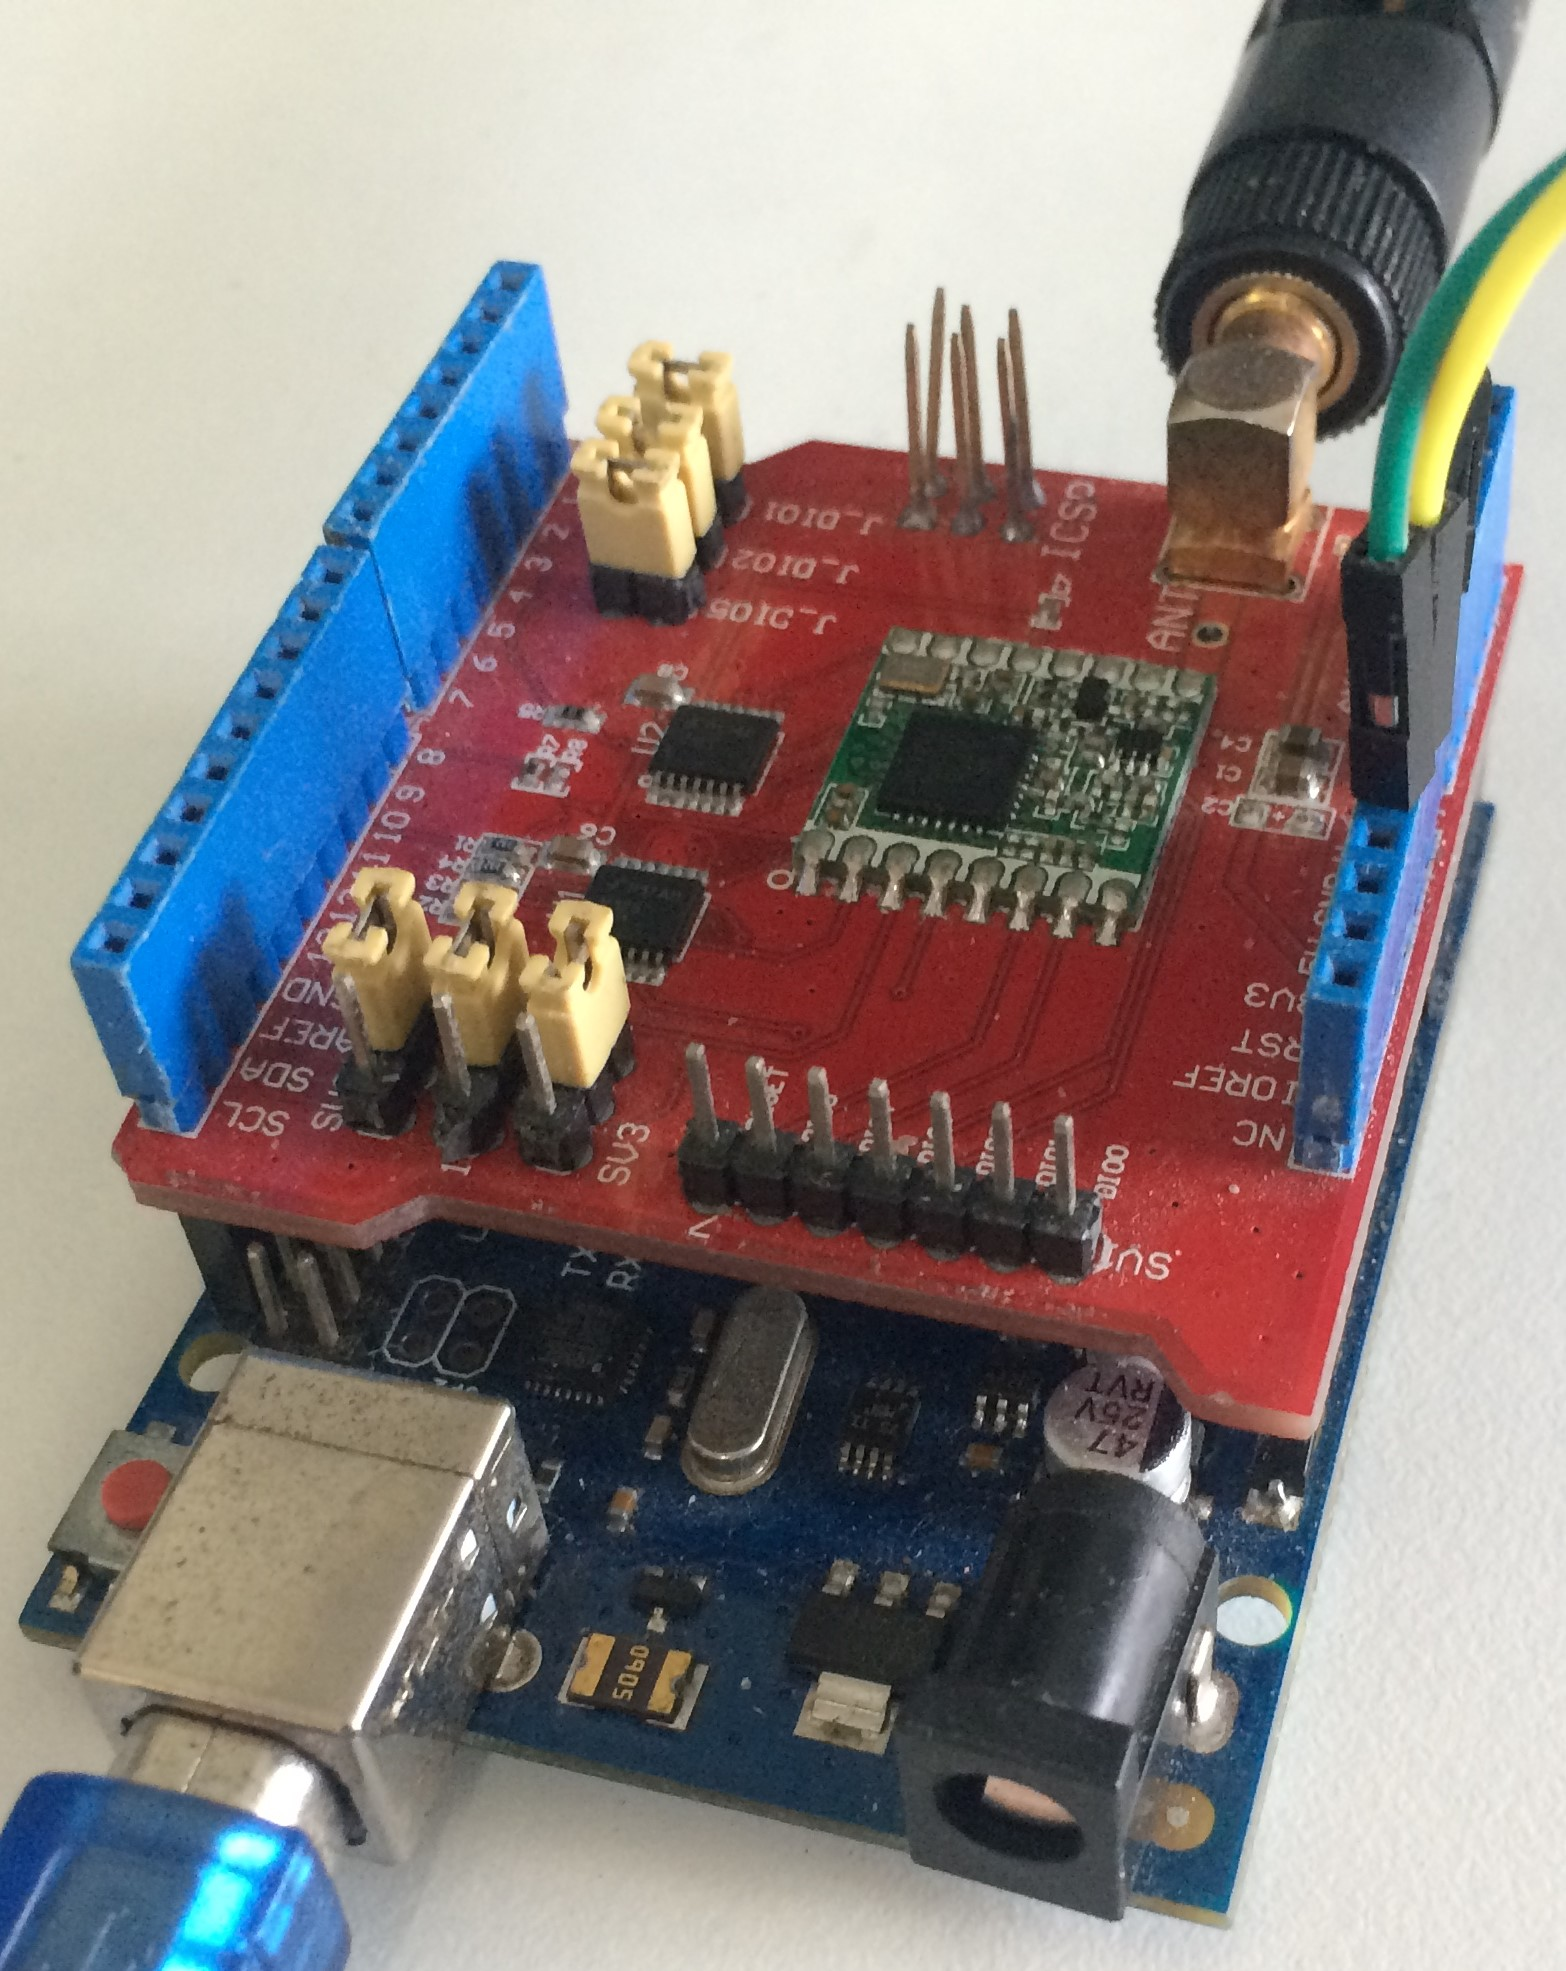
\includegraphics[scale=0.12]{image4/lora.jpg}
\end{center}
\caption{Gateway LoRa}
\end{figure}
\end{center}
Mạch \href{http://www.dragino.com/products/module/item/102-lora-shield.html}{LoRa Shield v1.3} kết hợp với mạch  \href{https://store.arduino.cc/usa/arduino-uno-rev3}{Arduino Uno R3} và sử dụng các cảm biến (sensor) - phụ thuộc vào nhu cầu mà sử dụng các loại cảm biến phù hợp.
\subsection{LoRa}
\label{chapterlora}
Điểm quan trọng của ứng dụng IoT yêu cầu chỉ truyền rất ít bit dữ liệu để theo dõi (monitor) các thiết bị tầm xa. Hệ thống mạng di động thì không phù hợp với vấn đề năng lượng pin (battery) và hiệu quả kinh tế khi gửi ít dữ liệu đi. Vì vậy, Low Power Wide Area Network (LPWAN) được đưa ra cho những ứng dụng này. LPWAN thích hợp cho việc gửi một lượng nhỏ dữ liệu với khoảng cách xa, trong khi thời lượng pin dài.
\begin{center}
\begin{figure}[htp]
\begin{center}

\includegraphics[scale=0.55]{image4/introlora.jpg}
\end{center}
\caption{Giới thiệu công nghệ LoRa \cite{tl15}}
\end{figure}
\end{center}
\subsubsection{LoRa là gì?}
LoRa™ \cite{tl14} (Long Range) là một kỹ thuật điều chế (modulation) dựa trên kỹ thuật Spread-Spectrum và một biến thể của Chirp Spread Spectrum (CSS), nó cho một khoảng cách xa hơn đáng kể cách kỹ thuật khác. Kỹ thuật không dây LoRa được phát triển bởi Cycleo SAS (sau này được mua lại bởi Semtech).

\subsubsection{LoRaWAN là gì?}
Điều chế LoRa nằm ở lớp vật lý (physical layer) của LoRaWAN, nó là một MAC protocol cho high capacity long range và Low Power Wide Area Networks (LPWAN). LoRa Alliance là một tổ chức mở phi lợi nhuận với các thành viên làm việc để chuẩn hóa LoRa Wide Area Network protocol (a.k.a LoRaWAN) cho LPWAN. LoRaWAN chú trong vào những nhu cầu cơ bản của IoT như bảo mật giao tiếp 2 chiều (bidirection communication), tính di động và các dịch vụ nội địa.\\
\begin{center}
\begin{figure}[htp]
\begin{center}
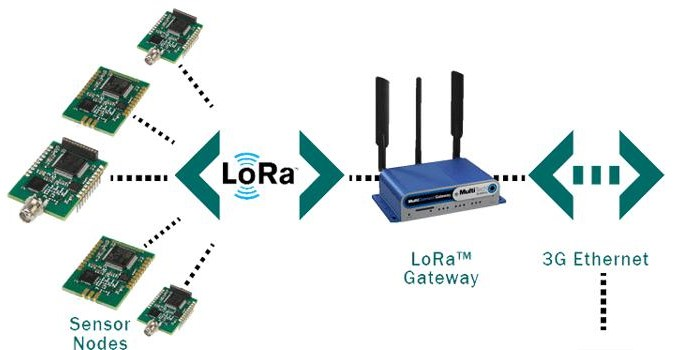
\includegraphics[scale=0.55]{image5/lora.jpg}
\end{center}
\caption{Giới thiệu LoRaWan}
\end{figure}
\end{center}
Hơn nữa, LoRaWAN network server quản lý data rate và RF output cho mỗi end-device một cách độc lập bằng giá trị trung bình (mean) của biểu đồ data rate thích nghi (adaptive data rate (ADR)), nó có thể mở rộng thời lượng pin và điều khiển thiết bị cuối lên tới 10 năm, và còn gia tăng tổng dung lượng network tới mức độc rất lớn.
\subsection{Arduino}
"Arduino là một bo mạch xử lý được dùng để lập trình tương tác với các thiết bị phần cứng như cảm biến, động cơ,… Điểm hấp dẫn ở Arduino với người lập trình là ngôn ngữ cực kì dễ học (giống C/C++), các ngoại vi trên bo mạch đều đã được chuẩn hóa, nên không cần biết nhiều về điện tử, chúng ta cũng có thể lập trình được những ứng dụng thú vị. Thêm nữa, vì Arduino là một platform đã được chuẩn hóa, nên đã có rất nhiều các bo mạch mở rộng (gọi là shield) để cắm chồng lên bo mạch Arduino, có thể hình dung nôm na là “library” của các ngôn ngữ lập trình." \cite{tl16}\\
\begin{center}
\begin{figure}[htp]
\begin{center}

\includegraphics[scale=0.1]{image4/arduinologo.png}
\end{center}
\caption{Giới thiệu Arduino}
\end{figure}
\end{center}
\newpage
Hiện tại, \href{http://arduino.vn/}{cộng đồng Arduino Việt Nam} và \href{https://www.arduino.cc/}{trên thế giới} là rất lớn mạnh. 

\section{Cài đặt công cụ hỗ trợ}
\subsection{Arduino IDE}
\begin{enumerate}
\item Truy cập vào địa chỉ \href{https://www.arduino.cc/en/Main/Software/}{https://www.arduino.cc/en/Main/Software/}. Bấm vào mục "Windows Installer, for Windows XP and up" để tải trực tiếp hoặc "Windows app" để tải thông qua Store.
\begin{center}
\begin{figure}[htp]
\begin{center}
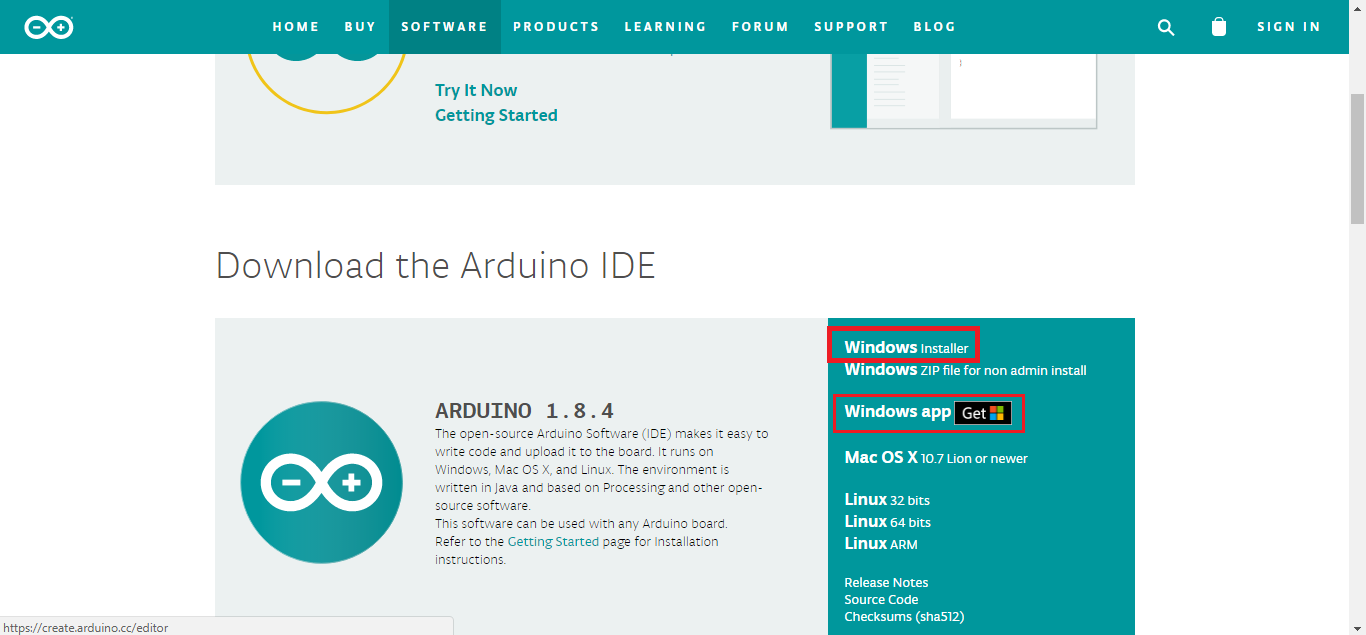
\includegraphics[scale=0.33]{image4/arduino1.png}
\end{center}
\caption{Truy cập trang \href{https://www.arduino.cc/en/Main/Software/}{tải Arduino}}
\end{figure}
\end{center}
\item Bấm "JUST DOWNLOAD" để tải bản cài đặt mới nhất cho Windows.
\begin{center}
\begin{figure}[htp]
\begin{center}
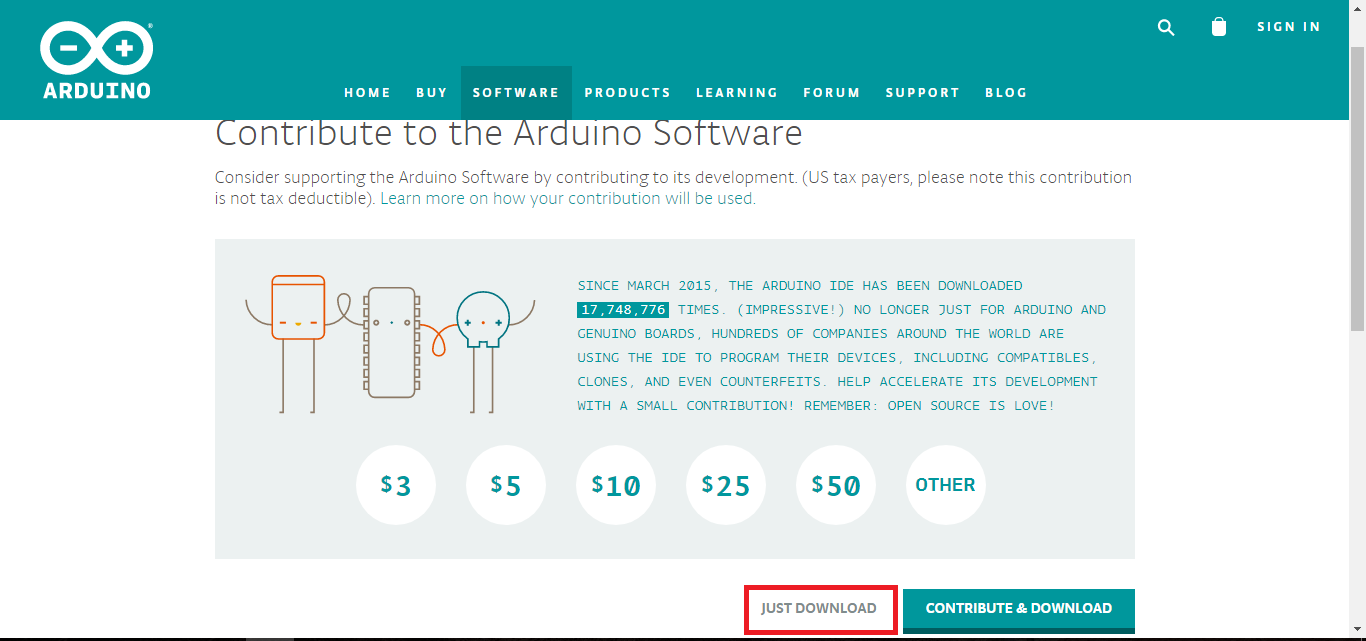
\includegraphics[scale=0.33]{image4/arduino2.png}
\end{center}
\caption{Chọn JUST DOWNLOAD}
\end{figure}
\end{center}
\item Tải về xong và khởi chạy file setup. Click "I Agree" đề đồng ý các điều khoản.
\begin{center}
\begin{figure}[htp]
\begin{center}
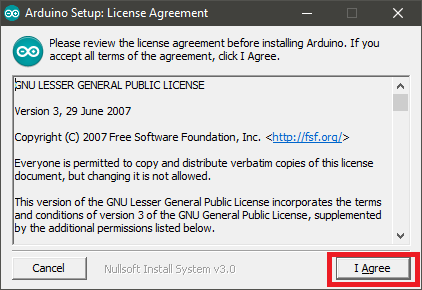
\includegraphics[scale=0.7]{image4/arduino3.png}
\end{center}
\caption{Chọn I Agree}
\end{figure}
\end{center}
\newpage
\item Chọn các công cụ cần cài đặt và "Next".
\begin{center}
\begin{figure}[htp]
\begin{center}
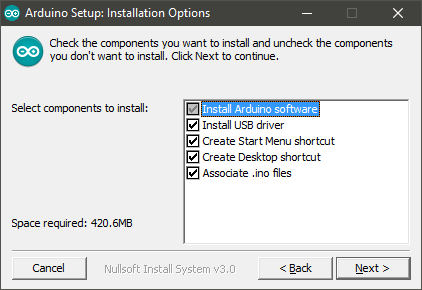
\includegraphics[scale=0.7]{image4/arduino4.PNG}
\end{center}
\caption{Chọn Next}
\end{figure}
\end{center}
\item  Chọn thư mục cài đặt Arduino IDE, đề nghị nên giữ mặc định thư mục cài đặt. Chọn "Install".
\begin{center}
\begin{figure}[htp]
\begin{center}
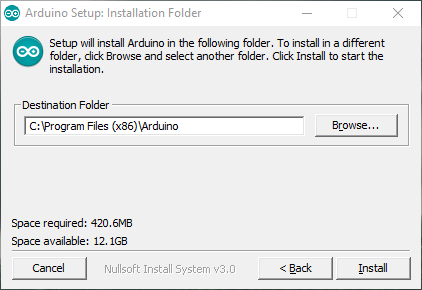
\includegraphics[scale=0.7]{image4/arduino5.PNG}
\end{center}
\caption{Chọn Install}
\end{figure}
\end{center}
\newpage
\item Chờ quá trình cài đặt hoàn tất.
\begin{center}
\begin{figure}[htp]
\begin{center}
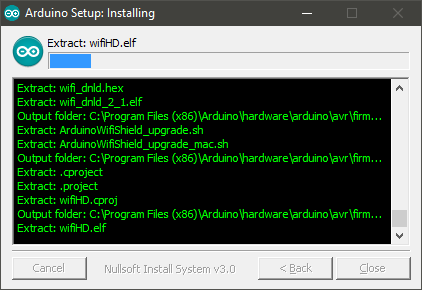
\includegraphics[scale=0.7]{image4/arduino6.PNG}
\end{center}
\caption{Chờ đợi cài đặt Arduino IDE}
\end{figure}
\end{center}
\item Khi cài gần xong, sẽ hiện các thông báo cài driver, bạn chỉ cần  tích vào "Always trust software from 'Adafruit Industries'" và chọn "Install".
\begin{center}
\begin{figure}[htp]
\begin{center}
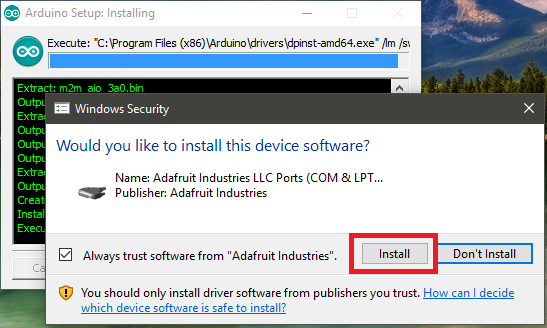
\includegraphics[scale=0.6]{image4/arduino7.png}
\end{center}
\caption{Chọn Install để cài đặt driver}
\end{figure}
\end{center}
\item Sau khi việc cài đặt driver kết thúc là đã cài đặt thành công Arduino IDE trên Windows.
\end{enumerate}
\subsection{Thêm thư viện RadioHead}
\begin{enumerate}
\item Truy cập vào địa chỉ \href{https://github.com/adafruit/RadioHead}{https://github.com/adafruit/RadioHead}. Nhấp vào "Clone or download" $\rightarrow$ chọn "Download ZIP".
\begin{center}
\begin{figure}[htp]
\begin{center}
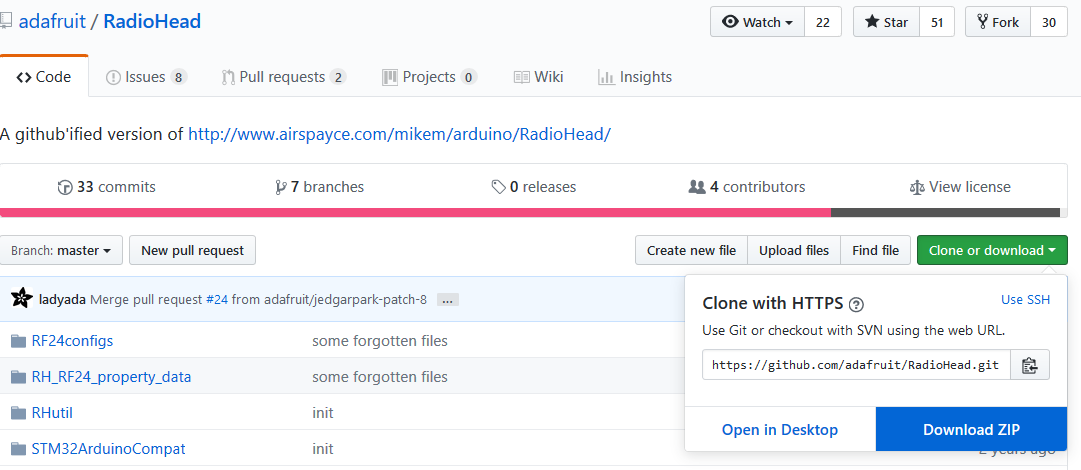
\includegraphics[scale=0.5]{image4/arduino8.png}
\end{center}
\caption{Tải tập thư viện từ \href{https://github.com/adafruit/RadioHead}{Github}}
\end{figure}
\end{center}
\item Tải về tập tin "RadioHead-master.zip".
\begin{center}
\begin{figure}[htp]
\begin{center}
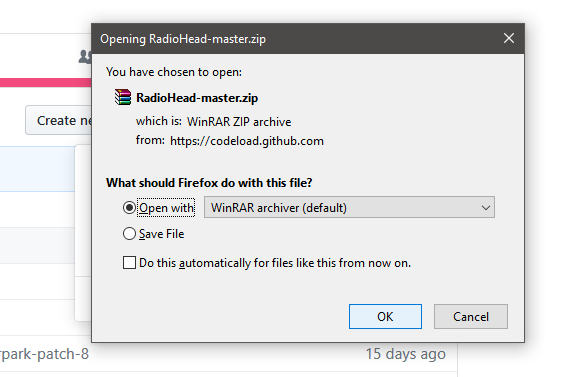
\includegraphics[scale=0.8]{image4/arduino9.png}
\end{center}
\caption{Nhấn OK để tải}
\end{figure}
\end{center}
\item Mở Arduino IDE, vào "Sketch" $\rightarrow$ "Include Library" $\rightarrow$ "Add .ZIP Library" để thêm tập tin thư viện.
\begin{center}
\begin{figure}[htp]
\begin{center}
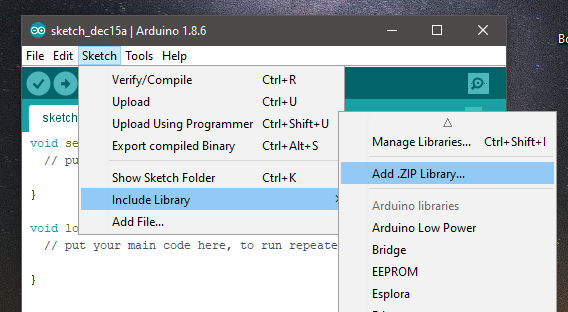
\includegraphics[scale=0.75]{image4/arduino10.png}
\end{center}
\caption{Thêm thư viện cho Arduino IDE}
\end{figure}
\end{center}
\item Chọn tập tin "RadioHead-master.zip" $\rightarrow$ nhấn "OK".
\begin{center}
\begin{figure}[htp]
\begin{center}
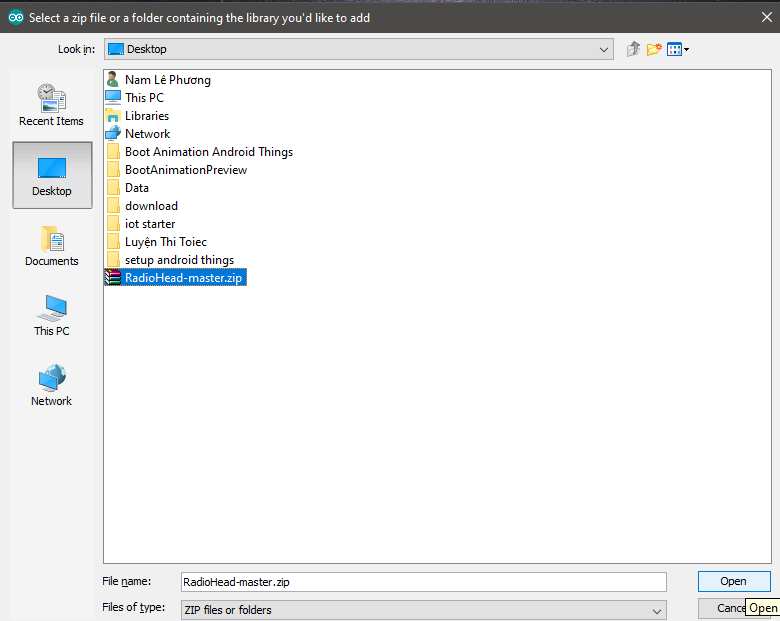
\includegraphics[scale=0.515]{image4/arduino11.png}
\end{center}
\caption{Chọn OK để thêm}
\end{figure}
\end{center}
\newpage
\item Vào "Sketch" $\rightarrow$ "Include Library" $\rightarrow$ tìm "RadioHead-master". Nếu đã có thì việc thêm thư viện đã hoàn tất.
\begin{center}
\begin{figure}[htp]
\begin{center}
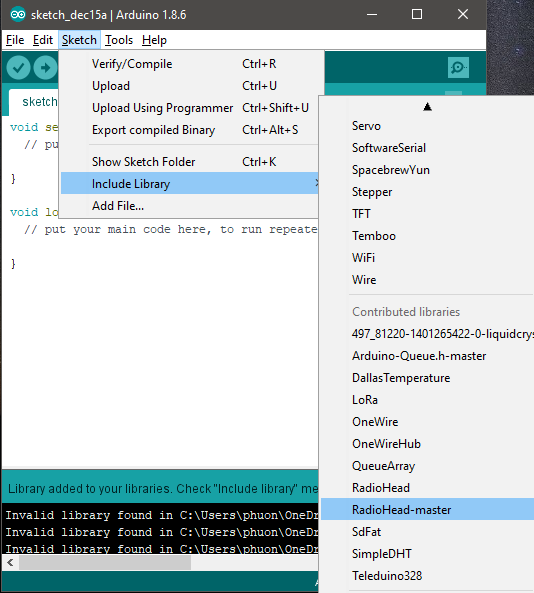
\includegraphics[scale=0.7]{image4/arduino12.png}
\end{center}
\caption{Kiểm tra thư viện đã được thêm}
\end{figure}
\end{center}
\end{enumerate}
\newpage
\section{Hướng dẫn chi tiết}
Nạp chương trình mẫu cho bên gửi gói tin (client).
\begin{enumerate}
\item Mở Arduino IDE, vào "File" $\rightarrow$ "Examples" $\rightarrow$ "RadioHead-master" $\rightarrow$ "rf95" $\rightarrow$ chọn "rf95\_client" để mở code mẫu của bên gửi gói tin.
\begin{center}
\begin{figure}[htp]
\begin{center}
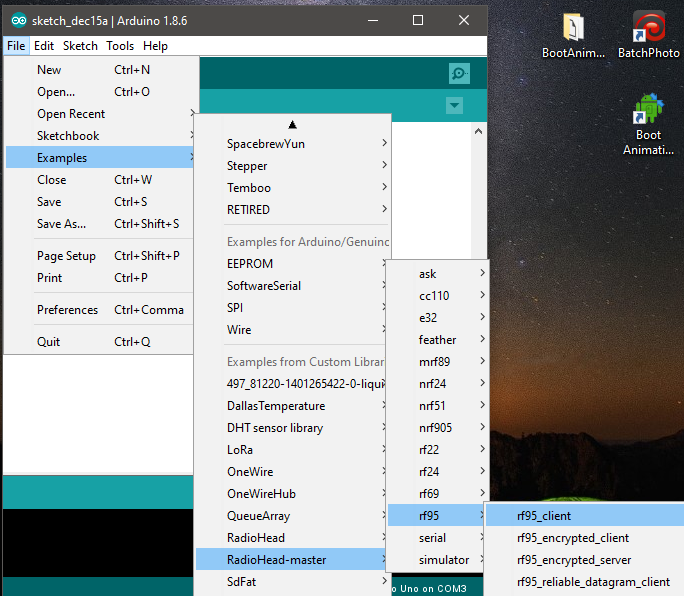
\includegraphics[scale=0.8]{image4/arduino13.png}
\end{center}
\caption{Mở code bên gửi "rf95\_client"}
\end{figure}
\end{center}
\newpage
\item Nhấn dấu mũi tên \textbf{$\Rightarrow$} hoặc "CTRL + U" để Upload code lên mạch.
\begin{center}
\begin{figure}[htp]
\begin{center}
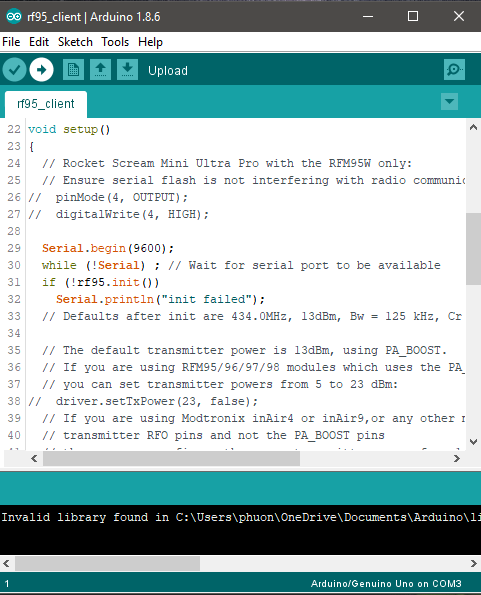
\includegraphics[scale=0.8]{image4/arduino14.png}
\end{center}
\caption{Nhấn dấu mũi tên \textbf{$\Rightarrow$} để Upload}
\end{figure}
\end{center}
\end{enumerate}
\newpage
Nạp chương trình mẫu cho bên nhận gói tin (server).
\begin{enumerate}
\item Mở Arduino IDE, vào "File" $\rightarrow$ "Examples" $\rightarrow$ "RadioHead-master" $\rightarrow$ "rf95" $\rightarrow$ chọn "rf95\_server" để mở code mẫu của bên nhận gói tin.
\begin{center}
\begin{figure}[htp]
\begin{center}
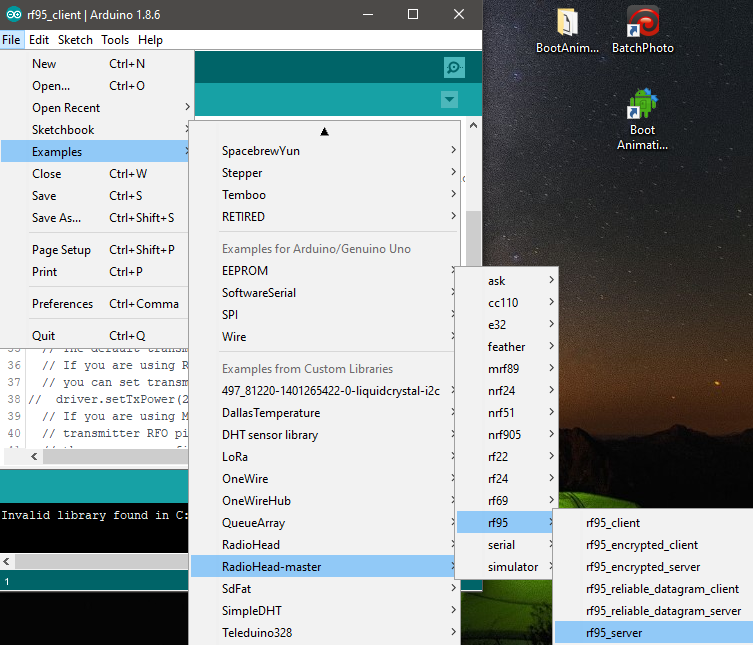
\includegraphics[scale=0.7]{image4/arduino15.png}
\end{center}
\caption{Mở code bên nhận "rf95\_server"}
\end{figure}
\end{center}
\newpage
\item Tại dòng thứ 22, đổi \lstinline{int led = 9;} thành \lstinline{int led = 8;} vì chân số 9 của LoRa Shield v1.3 là chân RESET.
\begin{center}
\begin{figure}[htp]
\begin{center}
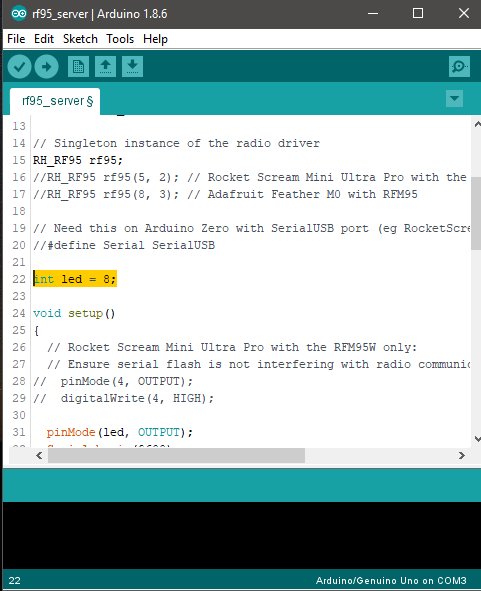
\includegraphics[scale=0.8]{image4/arduino16.png}
\end{center}
\caption{Thay đổi chân số 9 thành số 8}
\end{figure}
\end{center}
\newpage
\item Nhấn dấu mũi tên \textbf{$\Rightarrow$} hoặc "CTRL + U" để Upload code lên mạch.
\begin{center}
\begin{figure}[htp]
\begin{center}
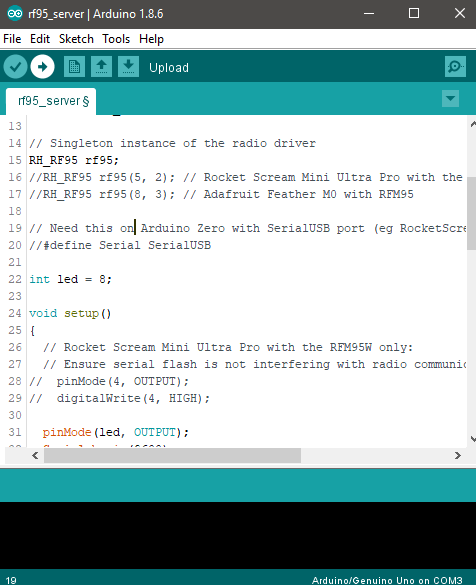
\includegraphics[scale=0.8]{image4/arduino17.png}
\end{center}
\caption{Nhấn dấu mũi tên \textbf{$\Rightarrow$} để Upload}
\end{figure}
\end{center}
\end{enumerate}
\section{Các lỗi thường gặp và cách khắc phục}
\begin{enumerate}
\item Lỗi cú pháp.\\
\textbf{Cách khắc phục:} Đọc phần gợi ý màu cam của chương trình để xem và sửa lỗi.
\begin{center}
\begin{figure}[htp]
\begin{center}
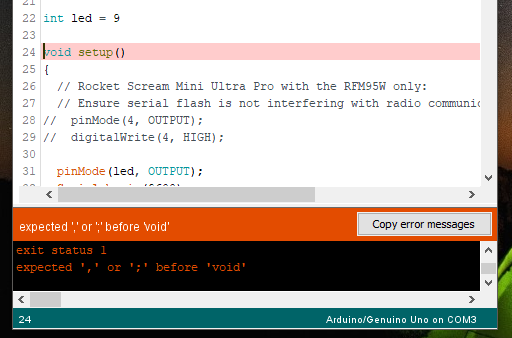
\includegraphics[scale=0.9]{image4/loi1.png}
\end{center}
\caption{Xem phần thông báo lỗi}
\end{figure}
\end{center}
\newpage
\item Lỗi logic.\\
\textbf{Cách khắc phục:} Xem xét lại tuần tự thực hiện lệnh, hướng đi đã hợp lý hay chưa.
\item Chọn sai board.\\
\textbf{Cách khắc phục:} Vào phần "Tools" $\rightarrow$ "Board" $\rightarrow$ kiểm tra board đã chọn là "Arduino/Genuino Uno".
\begin{center}
\begin{figure}[htp]
\begin{center}
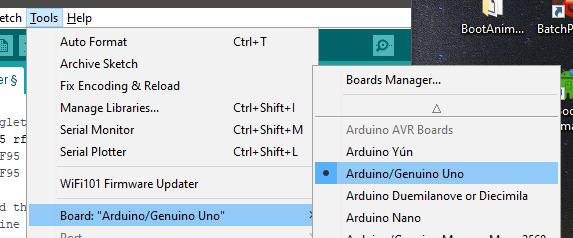
\includegraphics[scale=0.9]{image4/loi3.png}
\end{center}
\caption{Kiểm tra "Tools" $\rightarrow$ "Board: Arduino/Genuino Uno"}
\end{figure}
\end{center}
\item Chưa chọn Port.\\
\textbf{Cách khắc phục:} Vào phần "Tools" $\rightarrow$ "Port" hoặc "Serial Port" $\rightarrow$ kiểm tra đã chọn đúng Port chưa.
\begin{center}
\begin{figure}[htp]
\begin{center}
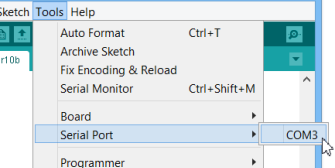
\includegraphics[scale=1.1]{image4/loi4.png}
\end{center}
\caption{Kiểm tra "Tools" $\rightarrow$ "Port" hoặc "Serial Port"}
\end{figure}
\end{center}
\item Chưa nối chân jump trên mạch.\\
\textbf{Cách khắc phục:} Nối tất cả 6 chân jump như \ref{pinjump} (các chân được khoanh khung màu vàng) thì LoRa mới có thể hoạt động.
\begin{center}
\begin{figure}[htp]
\begin{center}
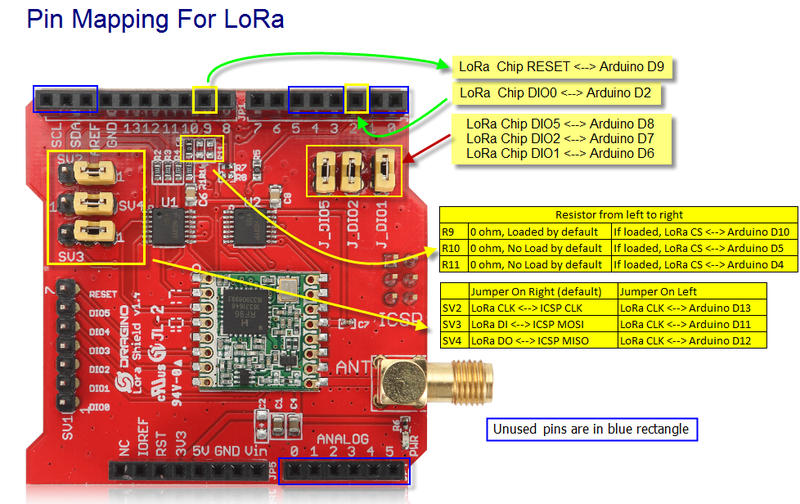
\includegraphics[scale=0.7]{image4/loi5.png}
\end{center}
\caption{Nối chân jump cho mạch LoRa}
\label{pinjump}
\end{figure}
\end{center}
\item Sử dụng nhầm chân RESET\\
\textbf{Cách khắc phục:} Không sử dụng chân số 9 với LoRa Shield v1.3 kết hợp với Arduino Uno R3 vì đó là chân reset của LoRa.
\item Cấu hình sai tần số hoạt động hoặc sai chế độ truyền dữ liệu.\\
\textbf{Cách khắc phục:} Nếu không thiết lập tần số thì cấu hình mặc định cho tần số và chế độ truyền là \lstinline{// Defaults after init are 434.0MHz, 13dBm, Bw = 125 kHz, Cr = 4/5, Sf = 128chips/symbol, CRC on}.\\
Tuy nhiên, có thể thay đổi bằng việc sử dụng các lệnh:
\begin{lstlisting}[label={list:sixth},caption=Các lệnh để thiết lập cấu hình]
setFrequency(434.0); //About 415~453MHz, default 434MHz
setTxPower(13); //Powers from 5 to 23 dBm, default 13dBm
setModemConfig(0); //Default 0
//0 < Bw = 125 kHz, Cr = 4/5, Sf = 128chips/symbol, CRC on. Medium range
//1 < Bw = 500 kHz, Cr = 4/5, Sf = 128chips/symbol, CRC on. Fast+short range
//2 < Bw = 31.25 kHz, Cr = 4/8, Sf = 512chips/symbol, CRC on. Slow+long range
//3 < Bw = 125 kHz, Cr = 4/8, Sf = 4096chips/symbol, CRC on. Slow+long range
\end{lstlisting}
Tham khảo các thông số cấu hình tại \href{https://www.semtech.com/uploads/documents/LoraDesignGuide\_STD.pdf}{đây} \cite{tl17}
\item Kích thước dữ liệu quá lớn.\\
\textbf{Cách khắc phục:} Nên lưu ý về kích thước tối đa của một gói tin là 256 bytes, trừ đi 4 bytes đầu (chứa các thông tin khác của gói tin) sẽ còn lại 252 bytes dành cho dữ liệu nội dung.
\item Ký tự kết thúc chuỗi dữ liệu\\
\textbf{Cách khắc phục:} Thường thì ký tự kết thúc chuỗi sẽ là '$\backslash$0' hoặc '$\backslash$r' hoặc '$\backslash$n'. Nên để ý khi thêm hoặc phân tích dữ liệu chuỗi trong một gói tin.
\item Kiểu dữ liệu.\\
\textbf{Cách khắc phục:} Do LoRa hoạt động trên thanh ghi, nên việc quản lý sẽ dựa vào chuỗi bit (từng byte). Vì thế tất cả các dữ liệu muốn gửi đi đều phải chuyển hóa thành từng \textbf{byte} hoặc chuỗi \textbf{char} hoặc kiểu số nguyên \textbf{int}.
\item Trùng gói tin khi có nhiều thiết bị gửi dữ liệu.\\
\textbf{Cách khắc phục:} Sử dụng các giao thức để quản lý như "Stop-n-wait", hàng đợi "Queue" \... và các giao thức quản lý khác giống trong network. 
\item Tham khảo cách khắc phục các lỗi thường gặp khác tại  \href{http://arduino.vn/reference/cac-loi-thuong-gap-tren-Arduino-va-cach-khac-phuc}{"http://arduino.vn/ reference/cac-loi-thuong-gap-tren-Arduino-va-cach-khac-phuc"}.
\end{enumerate}
\newpage
\section{Đo đạc hiệu suất của hệ thống}
%
%\subsection{Năng lượng tiêu thụ trung bình}
%
\subsection{Khoảng cách gửi nhận dữ liệu}
Dựa trên kết quả đo đạc thực tế, các thông số cấu hình đều sử dụng mặc định.
\begin{center}
\begin{table}[!h]
\begin{center}
\begin{tabular}{|c|c|c|c|}
\hline
\textbf{Lần} & \textbf{Điểm cố định} & \textbf{Điểm di động} & \textbf{Khoảng cách ước tính (m)}\\ 
\hline
1 & 105C6-CS1 & Solar Cafe-CS1 & 100\\
\hline
2 & 105C6-CS1 & Sân banh C2-CS1 & 150\\
\hline
3 & 420AH1-KTXA & Phía sau KTXXHH & 205\\
\hline
4 & 420AH1-KTXA & Sau nhà AG4-KTXA & 234\\
\hline
5 & 911AH1-KTXA & Tòa nhà H2-CS2 & 395\\
\hline
6 & 413AH1-KTXA & Tòa nhà H1-CS2 & 436\\
\hline
7 & 611H6-CS2 & Tòa nhà AH1-KTXA & 348\\
\hline
8 & 611H6-CS2 & Nhà Thi Đấu-CS2 & 264\\
\hline
9 & 709H6-CS2 & Tòa nhà AH1-KTXA & 378\\
\hline
10 & 709H6-CS2 & Nhà Thi Đấu-CS2 & 260\\
\hline
11 & 709H6-CS2 & Đường A4 & 430\\
\hline
12 & Sảnh tầng 7 H6-CS2 & Đại Học Quốc Tế & 432\\
\hline
\end{tabular}
\caption{Khoảng cách gửi nhận dữ liệu đo đạc được}
\label{dislora}
\end{center}
\end{table}
\end{center}
Từ bảng \ref{dislora}, trừ hao tổn năng lượng do vật cản (nhà, cây cối\...), ước lượng khoảng cách trung bình mà LoRa có thể gửi nhận với thông số cấu hình mặc định là \textbf{300m}, trong khoảng \textbf{250m - 350m}.\\
\textit{Khoảng cách có thể tăng thêm hoặc giảm nếu có sự thay đổi về cấu hình truyền nhận của LoRa.}
\subsection{Ước lượng thời gian hoạt động của node cảm biến}
Thời gian hoạt động có thể lên đến 10 năm khi sử dụng pin. \cite{tl18}